\documentclass{article}
\usepackage[german]{babel}
\usepackage[utf8]{inputenc}
\usepackage[a4paper,top=2cm,bottom=2cm,left=3cm,right=3cm,marginparwidth=1.75cm]{geometry}
\usepackage{amsmath}
\usepackage[onehalfspacing]{setspace}
\usepackage{graphicx}
    \graphicspath{ {./images/} }
\usepackage{url}
\usepackage{float}
\usepackage{pdfpages}
\usepackage{dirtytalk}
\usepackage{lastpage}
\usepackage{siunitx}
\sisetup{separate-uncertainty=true}
\usepackage{gensymb}
\usepackage{indentfirst}
\usepackage[square,numbers]{natbib}
\usepackage[colorlinks=true, allcolors=blue]{hyperref}
\usepackage[headsepline]{scrlayer-scrpage}
\pagestyle{scrheadings}
\clearpairofpagestyles
\begin{document}
\setcounter{totalnumber}{4}
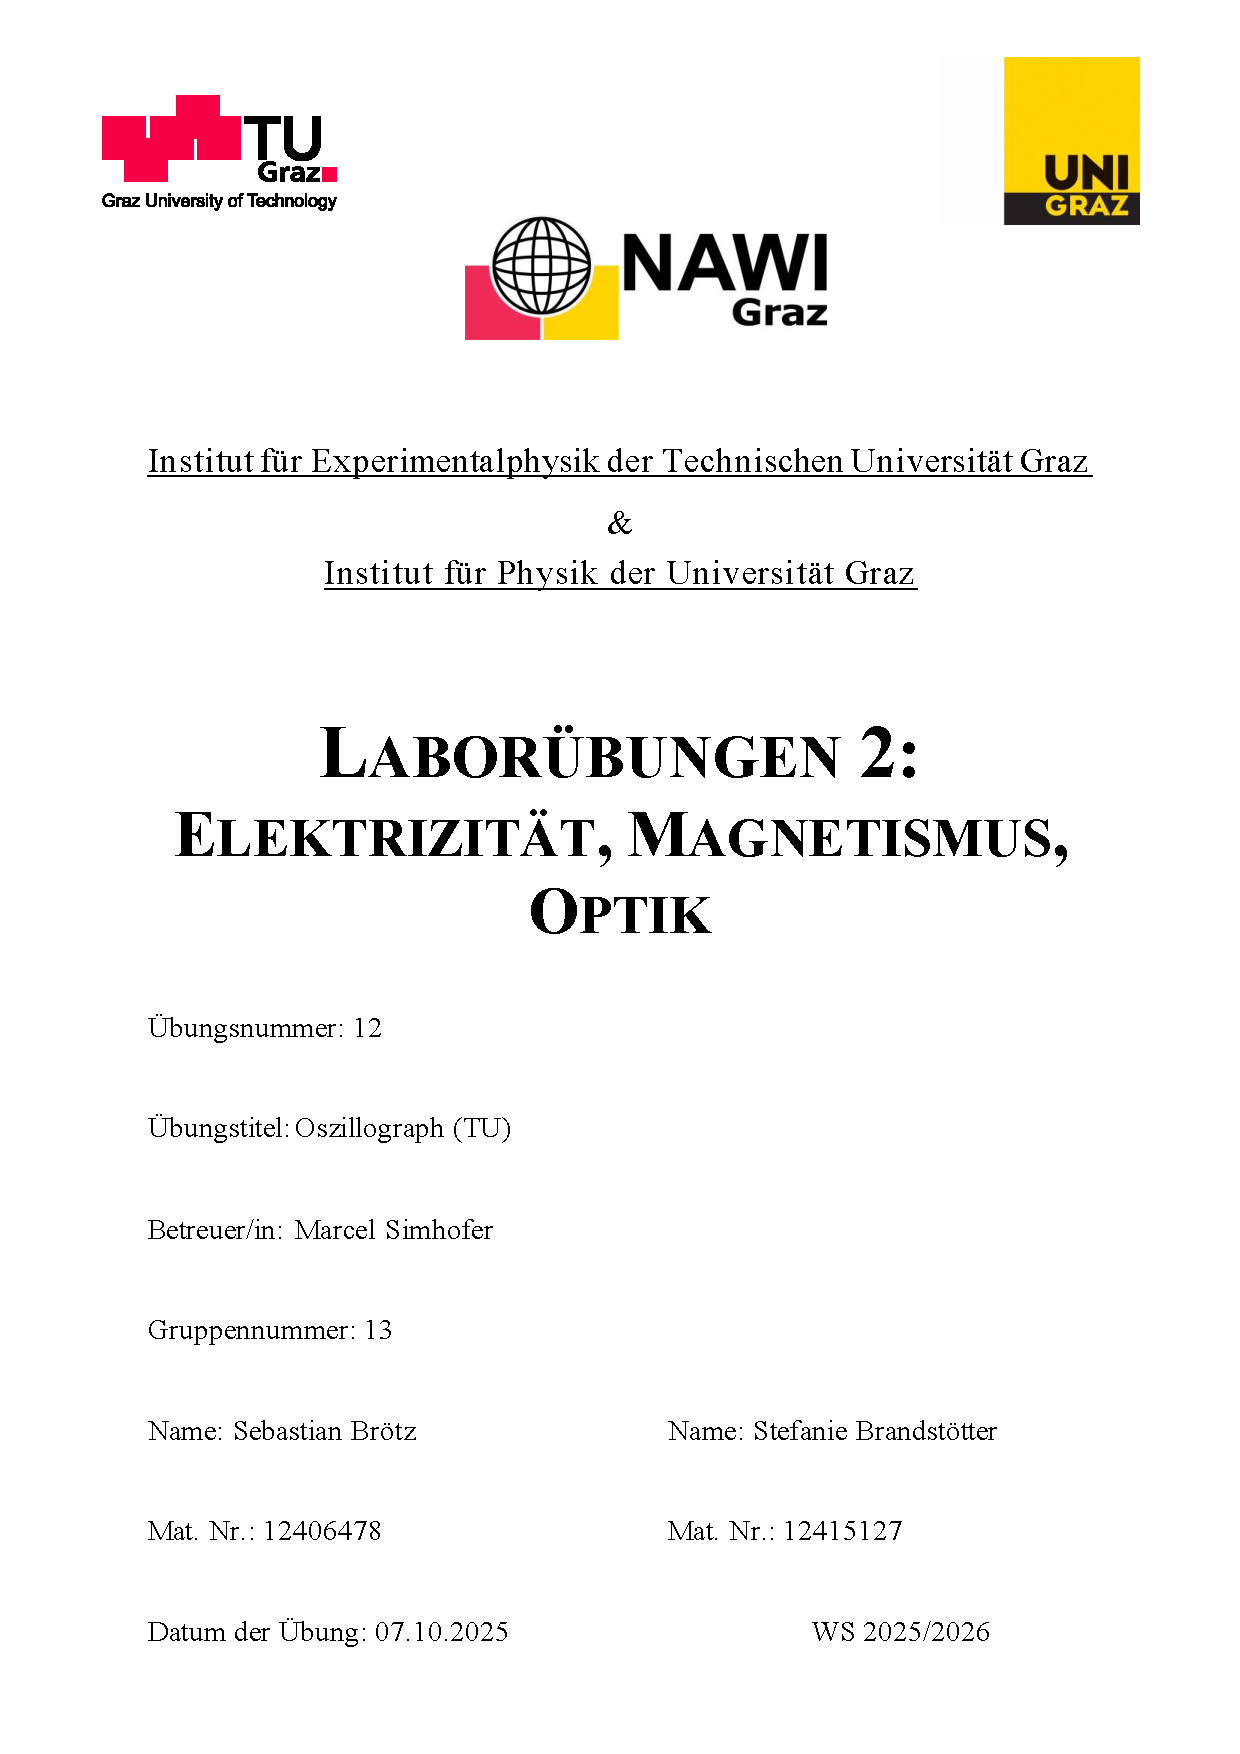
\includepdf{Deckblatt.pdf}

\ihead{Brandstötter, Brötz}
\chead{Erneuerbare Energien}
\ohead{14.10.2025}
\cfoot{\thepage{} / \pageref{LastPage}}

\tableofcontents
\newpage

\section{Auswertung}
% https://www.manualslib.com/manual/1051778/Mastech-Mas830l.html?page=7#manual
\subsection{Versuch 1: Photovoltaik}
\noindent In dem ersten Versuch wird das Verhalten einer Photovoltaik-Zelle untersucht. Dazu legt man an einer Lichtquelle eine fixe Spannung, in diesem Fall $U_q = 12{,}00 \; \text{V} \pm 1\%$ , an und misst die Leerlaufspannung $U_\text{leer}$ beziehungsweise den Kurzschlussstrom $I_\text{kurz}$ an der Photovoltaik-Zelle, welche in einem Fixen Abstand $d=(30{,}00 \pm 0{,}10) \; \text{cm}$ von der Lampe platziert wird. Das Photovoltaik-Modul besteht aus 2 einzelnen Zellen. Diese werden jeweils einmal einzeln vermessen, sowie in einer Parallelschaltung und einer Serienschaltung. Die gemessenen Leerlaufspannungen und Kurzschlussströme sind in Tabelle \ref{tab:MessungenWiderstand} angeführt.
\begin{table}[h]
    \centering
    \caption{Messergebnisse für die Leerlaufspannung $U_\text{leer}$ und den Kurzschlussstrom $I_\text{kurz}$ eines Photovoltaik-Moduls für eine Parallel- und Serienschaltung, sowie für die einzelne Verschaltung der Zellen selbst.}
    \label{tab:MessungenWiderstand}
    \begin{tabular}{c|c|c}
    Messung & $U_{\text{leer}}$ / V & $I_{\text{kurz}}$ / mA \\\hline
    Links & $1{,}160 \pm 0{,}010$ & $29{,}3 \pm 0{,}8$ \\
    Rechts & $1{,}127 \pm 0{,}010$ & $29{,}6 \pm 0{,}8$ \\
    Parallel & $1{,}128 \pm 0{,}010$ & $57{,}9 \pm 1{,}2$ \\
    Serie & $2{,}17 \pm 0{,}05$ & $31{,}2 \pm 0{,}8$ \\
    \end{tabular}
\end{table}

\noindent Für den zweiten Teil dieses Versuches wird das Modul in Serie verschalten und bei verschiedenen Abständen $d$ die Leerlaufspannung und der Kurzschlussstrom aufgezeichnet. Die entsprechenden Messergebnisse sind in Abbildung \ref{fig:V1_PV_Kennlinien} dargestellt.

\begin{figure}[H]
    \centering
    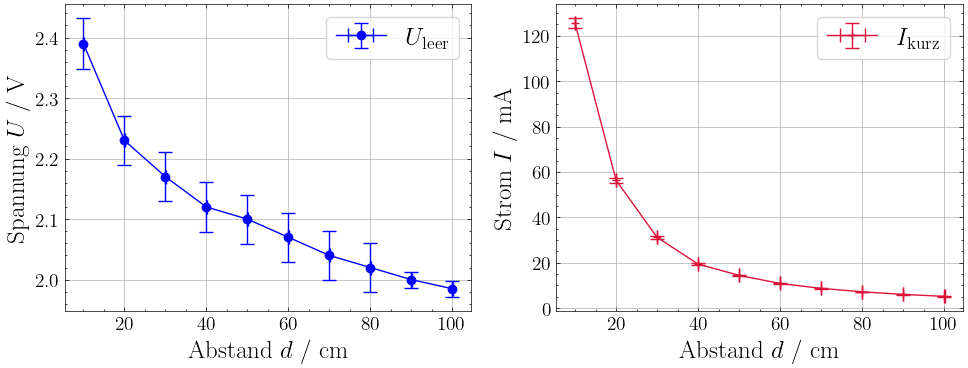
\includegraphics[width=0.9\linewidth]{images/V1_Photovoltaik_Kennlinien.png}
    \caption{Aufgezeichnete Leerlaufspannungen $U_\text{leer}$ (blau) und Kurzschlussströme $I_\text{kurz}$ (rot) eines Photovoltaik-Moduls in Serienschaltung bei verschiedenen Abständen $d$ zu einer Lichtquelle.}
    \label{fig:V1_PV_Kennlinien}
\end{figure}

\subsection{Versuch 2: Brennstoffzelle}
\subsubsection{Bestimmung des Wirkungsgrades}
\noindent Im zweiten Versuch wird eine elektrische Schaltung, wie in Abbildung \ref{fig:V2_BZ_Schaltplan} dargestellt, aufgebaut um den Wirkungsgrad $\eta$ einer Brennstoffzelle zu bestimmen.

\begin{figure}[h!]
    \centering
    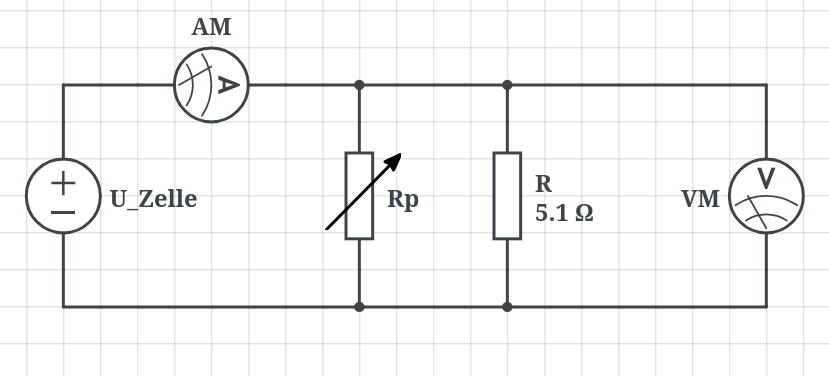
\includegraphics[width=0.7\linewidth]{images/V2_Schaltplan_BZ.png}
    \caption{Elektrischer Schaltplan entsprechend der Angabe \cite{Angabe} zur Bestimmung des Wirkungsgrades $\eta$ einer Brennstoffzelle. Die verwendeten Bauteile umfassen: eine Brennstoffzelle $U_\text{Zelle}$, ein Potenziometer $U_p$, einen Widerstand $R=5{,}1 \; \Omega$, ein Spannungsmessgerät $VM$ und ein Strommessgerät $AM$.}
    \label{fig:V2_BZ_Schaltplan}
\end{figure}

% Steffi bitte hier schreiben wiso nicht 6ml -> wegen kaputter Widerstand
% Allgemein die Werte sind kompletter müll.
\noindent Die Brennstoffzelle wird gemäß der Angabe \cite{Angabe} präpariert, und gemäß der Schaltung so lange betrieben, bis $2 \; \text{ml}$ Wasserstoff ($H_2$) in elektrische Energie umgesetzt wurden. Dabei werden die Zeit $t_\text{diff}$ für diesen Prozess, der Strom $I$ und die Spannung $U$ bei Erreichen des finalen Volumens gemessen. Die Zahlenwerte ergeben sich dabei zu:
$$t_\text{diff} = (350 \pm 10) \; \text{s} \qquad \qquad U = (80 \pm 4) \; \text{mV} \qquad \qquad I = (15{,}4 \pm 0{,}3) \; \text{mA}$$
Die Unsicherheit für die Zeitmessung wurde hier aufgrund der geringen Genauigkeit bei der Bestimmung des Volumens zu $\Delta t_\text{diff} = 10 \; \text{s}$ gewählt. Aus diesen Werten kann nun die elektrische Leistung $P_\text{el}$ , sowie die gelieferte elektrische Energie $E_\text{el}$ der Brennstoffzelle bestimmt werden.
\begin{equation}\label{eq:Pel}
    P_\text{el} = U\cdot I\qquad \qquad\qquad E_\text{el} = P_\text{el}\cdot t_\text{diff}.
\end{equation}
Aus Gleichung \ref{eq:Pel} ergeben sich die folgenden Werte, wobei die Unsicherheit der beiden Größen über die Größtunsicherheitsmethode berechnet wird.
$$P_\text{el} = (1{,}23 \pm 0{,}07) \; \text{mW} \qquad \qquad \qquad E_\text{el} = (430 \pm 40)\; \text{mJ}$$

\noindent Als Vergleich dazu lässt sich die chemische Energie des verbrauchten Wasserstoffs berechnen. Dafür benötigt man einerseits die Stoffmenge $n_{H_2}$, welche durch Gleichung \ref{eq:Stoffmenge} gegeben ist.
\begin{equation}\label{eq:Stoffmenge}
    n_{H_2} = \frac{\Delta V}{V_\text{mol}}
\end{equation}
\noindent Hier ist $\Delta V = 2 \; \text{ml}$ die gemessene Volumendifferenz und $V_\text{mol}$ das Molvolumen des Wasserstoffs. Für die Normalbedingungen von einer \say{Temperatur von $298 \; \text{K}$ ($24{,}85$ °C) und einem Druck von $1$ atm ($1{,}0133\cdot 10^5$ Pascal)}\cite{Molvolumen} gilt für das Molvolumen von Wasserstoff $V_\text{mol}= 22{,}4135 \; \text{l}\,\text{mol}^{-1}$. Zur Berechnung der chemischen Energie benötigt man zusätzlich noch die Reaktionsenthalpie der Wasserbildung \cite{NISTWater}, welche sich zu $H_R =  285{,}8\;\text{kJ}\,\text{mol}^{-1}$ ergibt.\\
Die chemisch verfügbare Energie des verbrauchten Wasserstoffs berechnet sich aus dem Produkt der Stoffmenge und der Reaktionsenthalpie. Aus der Berechnung ergibt sich dabei:
$$E_\text{chem} = n_{H_2}\cdot H_\mathrm{R} \qquad \rightarrow \qquad E_\text{chem} = (26 \pm 3) \; \text{J}$$

\noindent Schlussendlich kann der Wirkungsgrad \(\eta\) der Brennstoffzelle aus dem Verhältnis der geleisteten elektrischen Energie zu der benötigten chemischen Energie berechnet werden.
\begin{equation}
    \eta = \frac{E_\text{el}}{E_\text{chem}} \qquad \rightarrow \qquad \eta = (1{,}7 \pm 0{,}4) \; \%
\end{equation}
Die Unsicherheit der Zahlenwerte für die chemische Energie und den Wirkungsgrad folgt in den obigen Rechnungen aus der Größtunsicherheitsmethode.
\subsubsection{Bestimmung der Kennlinie}
\noindent Für die Brennstoffzelle soll nun eine Storm-Spannungs-Kennlinie sowie die gelieferte Leistung $P$ bestimmt werden. Dabei wird die Schaltung aus Abbildung \ref{fig:V2_BZ_Schaltplan} verwendet, um die Spannung $U$ und den Strom $I$ bei verschiedenen Widerstandswerten aufzuzeichnen. Diese Messungen sind in Abbildung \ref{fig:V2_BZ_Kennlinien_Messung} einerseits für Messungen ohne den konstanten Widerstand $R$ in blau und andererseits mit Widerstand in rot dargestellt.
\begin{figure}[H]
    \centering
    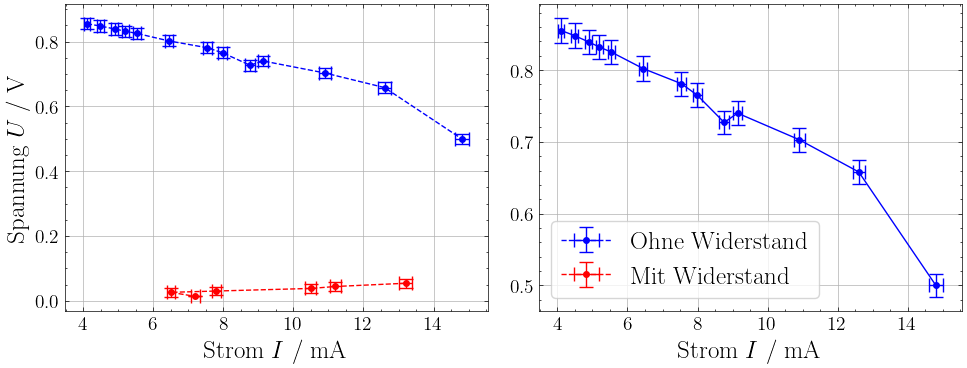
\includegraphics[width=0.9\linewidth]{images/V2_BZelle_2_Kennlinie_Messung.png}
    \caption{Gemessene Kennlinie der Brennstoffzelle: Spannung \(U\) in Abhängigkeit vom Strom \(I\) einerseits für Messungen ohne zusätzlichen Widerstand $R$ in blau und andererseits mit parallel gestaltetem Widerstand in rot. Der rechte Plot zeigt zudem noch eine Detailansicht der Messungen ohne Widerstand.}
    \label{fig:V2_BZ_Kennlinien_Messung}
\end{figure}

\noindent Als nächster Schritt soll in dem linearen Teil der Kennlinie eine Ausgleichsgerade berechnet werden, um die Steigung $R_\text{in}$ in diesem Bereich zu bestimmen. Dieser Schritt ist in Grafik \ref{fig:V2_BZ_lin_fit_Spannung} zu erkennen.
\begin{figure}[H]
    \centering
    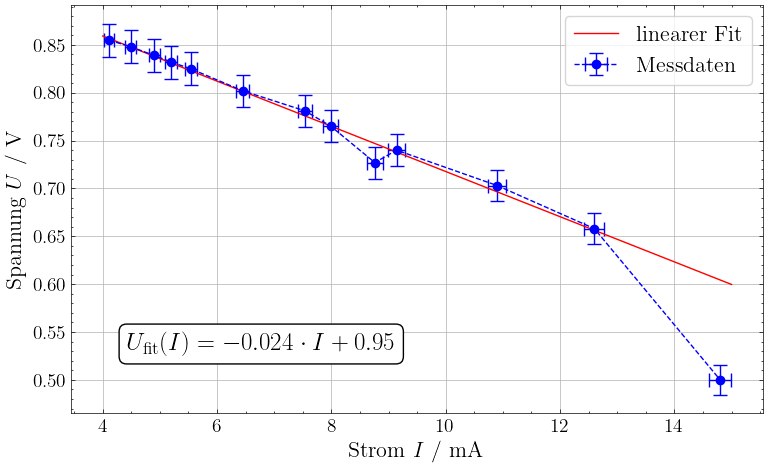
\includegraphics[width=0.6\linewidth]{images/V2_BZelle_2_Kennlinie_Fit_U.png}
    \caption{Linearer Fit des linearen Bereichs der Spannungs-Strom-Kennlinie. Die Ausgleichsgerade ist in rot und die Messdaten sind in blau dargestellt. Die Steigung \(R_\text{in}\) und der Achsenabschnitt \(U_0\) können aus der Regressionsrechnung entnommen werden.}
    \label{fig:V2_BZ_lin_fit_Spannung}
\end{figure}
\noindent Für die Ausgleichsgerade ergeben sich die Steigung $R_\text{in}$ und der Achsenabschnitt $U_0$ aus der Regressionsrechnung.
$$U_\text{fit}(I) = -R_\text{in} \cdot I + U_0 = -0{,}024 \cdot I + 0{,}95$$
Außerdem wird die Leistung $P=U\cdot I$ in Abhängigkeit vom Strom $I$ für jeden Messpunkt berechnet und eine quadratische Ausgleichskurve an die Datenpunkte angepasst. In Abbildung \ref{fig:V2_BZ_quad_fit_Leistung} sind die berechneten Punkte und die quadratische Funktion angezeigt.
\begin{figure}[H]
    \centering
    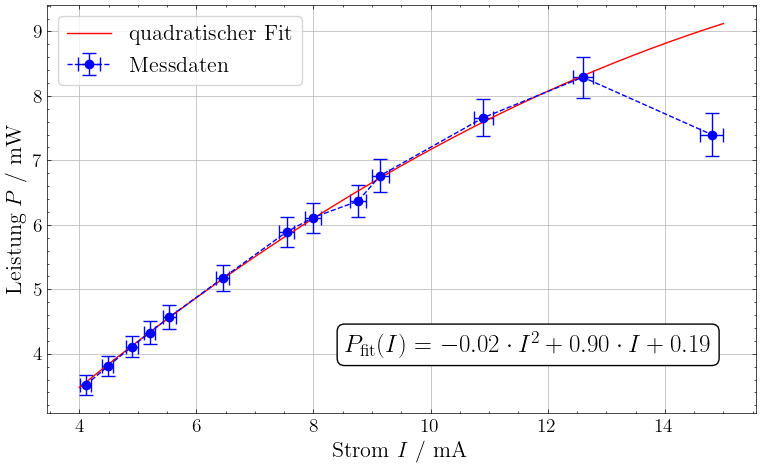
\includegraphics[width=0.6\linewidth]{images/V2_BZelle_2_Kennlinie_Fit_P.png}
    \caption{Leistung \(P=U\cdot I\) in Abhängigkeit vom Strom \(I\). Darstellung mit quadratischem Fit in rot und Messdaten in blau.}
    \label{fig:V2_BZ_quad_fit_Leistung}
\end{figure}
\noindent Aus der Regressionsrechnung \cite{Fit} ergibt sich ein quadratischer Zusammenhang der Messdaten in der Form von:
$$P_\text{fit}(I) = A \cdot I^2 + B\cdot I + C = -0{,}02 \cdot I^2 + 0{,}90 \cdot I + 0{,}19$$

\subsection{Versuch 3: Windkraft}
\noindent Als dritter Teil des Erneuerbare-Energien Versuchs wird die Windenergie betrachtet. Hierzu platziert man ein Windrad in einem Abstand von $d=(5{,}00 \pm 0{,}10) \; \text{cm}$ hinter einem Windgenerator und erzeugt verschiedene Windstärken durch variieren der Gleichspannung $U_\text{M}$ der Windmaschine.
Die Messungen für die Leerlaufspannung $U_\text{leer}$ am Windrad der unterschiedlichen Windstärken sind in Abbildung \ref{fig:V3_WK_fixer_Abstand} angezeigt.
\begin{figure}[h!]
    \centering
    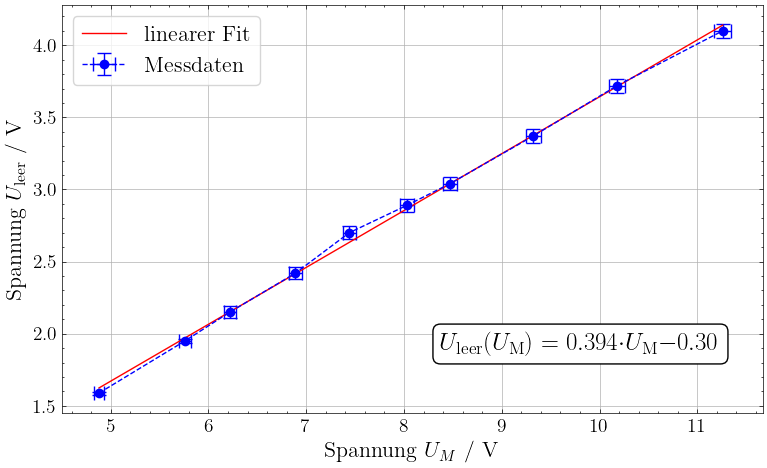
\includegraphics[width=0.6\linewidth]{images/V3_Windkraft_fixerAbstand.png}
    \caption{Messungen der Leerlaufspannung $U_\text{leer}$ eines Windrades bei verschiedenen Windstärken. Die Windstärke entspricht in dem Versuch der angelegten Gleichspannung $U_M$ an der Windmaschine. Zu erkennen sind einerseits die Messdaten mit Unsicherheit in blau und eine Ausgleichsgerade in rot.}
    \label{fig:V3_WK_fixer_Abstand}
\end{figure}

\noindent Die Form der Ausgleichsgerade für die Leerlaufspannung $U_\text{leer}$ in Abhängigkeit von der Spannung der Windmaschine $U_\text{M}$ ergibt sich dabei zu:
$$U_\text{leer}(U_\text{M}) = 0{,}39 \cdot U_\text{M} - 0{,}30 \qquad \qquad U_\text{leer} (10{,}06) = (3{,}68 \pm 0{,}05) \; \text{V}$$
Ebenfalls soll das Verhalten bei verschiedenen Abständen zwischen Windrad und Generator untersucht werden. Dabei wird eine fixe Erzeugerspannung $U_\text{M} =10{,}09 \; \text{V} \pm 1 \%$ eingestellt und die Leerlaufspannung bei unterschiedlichen Abständen $d$ gemessen.
Bei der Versuchsdurchführung wurde kein Messpunkt für $d=5\; \text{cm}$ aufgezeichnet, weshalb dieser mit einer Regressionsrechnung aus dem vorigen Versuch bestimmt wird. Die Unsicherheit der berechneten Spannung bei $d=5 \; \text{cm}$ folgt ebenfalls aus der Regressionsrechnung.
Der rechnerisch ermittelte Wert und die Messwerte der Leerlaufspannung bei den verschiedenen Abständen sind in Abbildung \ref{fig:V3_WK_fixe_Spannung} ersichtlich.

\begin{figure}[H]
    \centering
    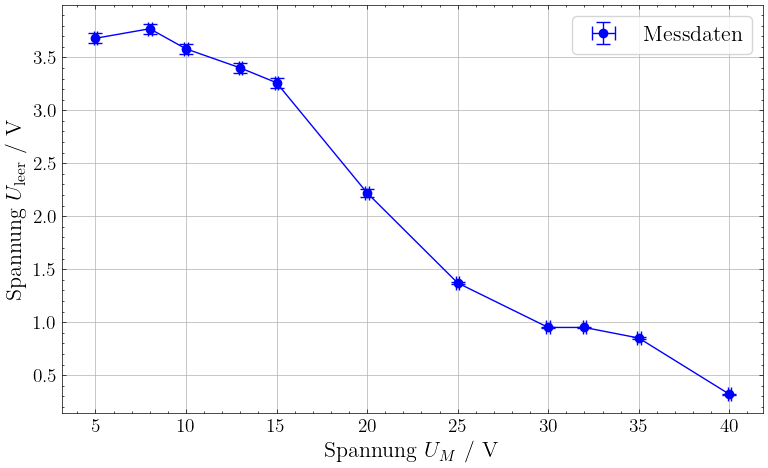
\includegraphics[width=0.6\linewidth]{images/V3_Windkraft_fixeSpannung.png}
    \caption{Gemessene Leerlaufspannungen $U_\text{leer}$ des Windrades in Abhängigkeit vom Abstand $d$ zur Windmaschine. Dargestellt sind die Messwerte (blaue Punkte) inklusive Messunsicherheiten sowie ein rechnerisch bestimmter Wert (gelber Punkt) für $d=5 \; \text{cm}$, der aus einer Regressionsrechnung ermittelt wurde.
    Während des gesamten Experiments wurde der Windgenerator mit einer konstanten Erzeugerspannung $U_M$ betrieben.}
    \label{fig:V3_WK_fixe_Spannung}
\end{figure}

\noindent Im weiteren Verlauf des Windkraft Versuchs gilt es die Speicherung der erzeugten Windenergie zu analysieren. Dabei werden ein Kondensator $C$ und eine Brennstoffzelle als Energiespeicher betrachtet und anschließend in der Diskussion verglichen.
\subsubsection{Energiespeicher: elektrisches Potenzial}
\noindent Zuerst wird die Speicherung der Energie des Windrades in Form eines elektrischen Potenzials betrachtet. Dazu wird eine fixe Spannung an der Windmaschine $U_\text{M}$ angelegt und das Windrad in einem Abstand $d$ dazu platziert. An das Windrad wird ein Kondensator angeschlossen und die Spannung über diesen, genannt $U_C$, für das Verhalten bei plötzlichem Einschalten oder Unterbrechen des Windes aufgezeichnet. In den folgenden drei Abbildungen \ref{fig:V3_WK_Fit1}, \ref{fig:V3_WK_Fit2} und \ref{fig:V3_WK_Fit3} ist jeweils zweimal das Aus- und zweimal das Einschaltverhalten für drei verschiedene Kondensatoren dargestellt. Die Messreihe aus Abbildung \ref{fig:V3_WK_Fit1} gehört dabei zu Kondensator $A$, Abbildung \ref{fig:V3_WK_Fit2} zu Kondensator $B$ und Abbildung \ref{fig:V3_WK_Fit3} zu Kondensator $C_1$ mit bekannter Kapazität $C_1 = 1 \; \text{F} \pm 1\%$.

\begin{figure}[H]
    \centering
    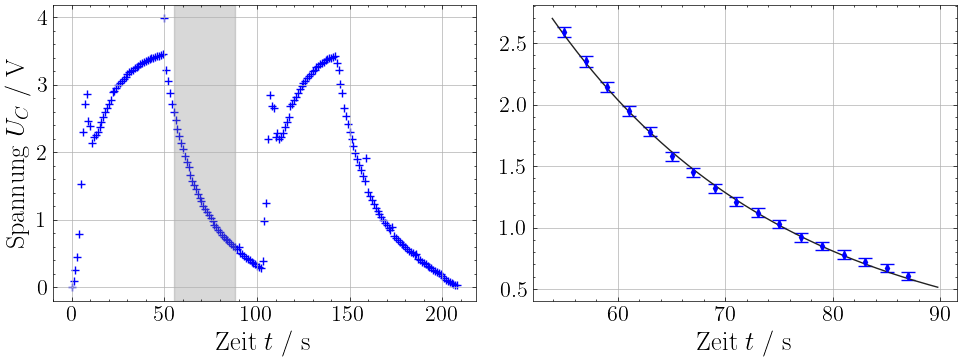
\includegraphics[width=0.95\linewidth]{images/V3_Windkraft_Fit_Mess1.png}
    \caption{\textbf{Linker Plot}: Gemessene Kondensatorspannung $U_C$ beim Ein- und Ausschaltvorgang des Windrades. Dargestellt sind jeweils zwei Messungen für das Lade- und Entladeverhalten von Kondensator $A$. \textbf{Rechter Plot}: Exponentielle Ausgleichsfunktion in schwarz dargestellt, angepasst an einen ausgewählten Entladeabschnitt (grauer Bereich) zur Bestimmung der Zeitkonstante $\tau$. }
    \label{fig:V3_WK_Fit1}
\end{figure}

\begin{figure}[H]
    \centering
    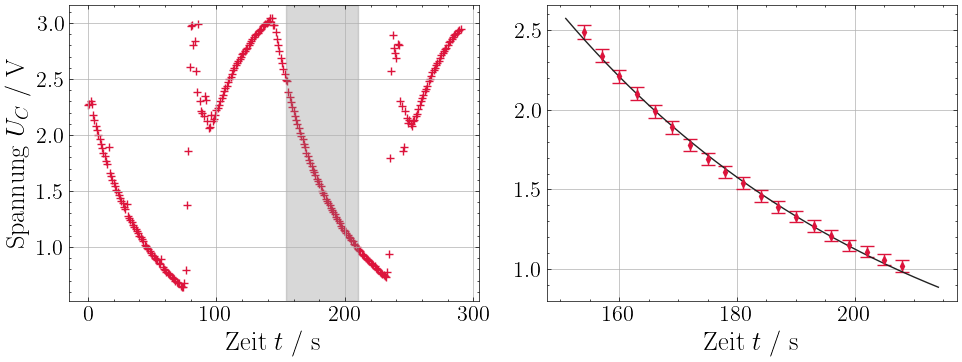
\includegraphics[width=0.95\linewidth]{images/V3_Windkraft_Fit_Mess2.png}
    \caption{\textbf{Linker Plot}: Gemessene Kondensatorspannung $U_C$ beim Ein- und Ausschaltvorgang des Windrades. Dargestellt sind jeweils zwei Messungen für das Lade- und Entladeverhalten von Kondensator $B$. \textbf{Rechter Plot}: Exponentielle Ausgleichsfunktion in schwarz dargestellt, angepasst an einen ausgewählten Entladeabschnitt (grauer Bereich) zur Bestimmung der Zeitkonstante $\tau$. }
    \label{fig:V3_WK_Fit2}
\end{figure}

\begin{figure}[H]
    \centering
    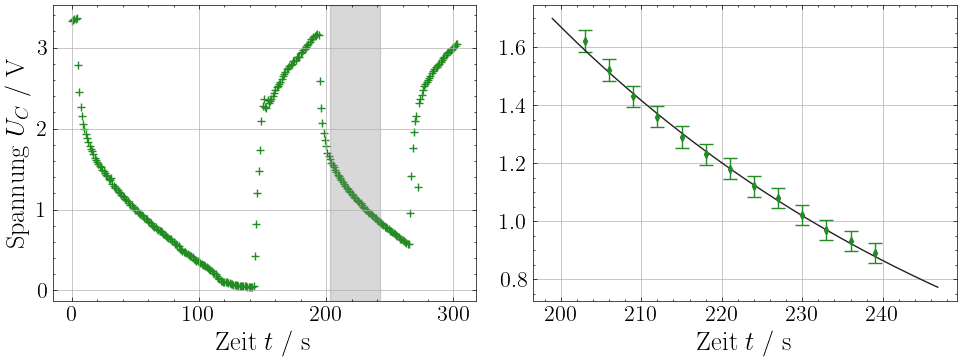
\includegraphics[width=0.95\linewidth]{images/V3_Windkraft_Fit_Mess3.png}
    \caption{\textbf{Linker Plot}: Gemessene Kondensatorspannung $U_C$ beim Ein- und Ausschaltvorgang des Windrades. Dargestellt sind jeweils zwei Messungen für das Lade- und Entladeverhalten von Kondensator $C_1 = 1 \; \text{F}$. \textbf{Rechter Plot}: Exponentielle Ausgleichsfunktion in schwarz dargestellt, angepasst an einen ausgewählten Entladeabschnitt (grauer Bereich) zur Bestimmung der Zeitkonstante $\tau$.}
    \label{fig:V3_WK_Fit3}
\end{figure}

\noindent Für jede der drei Messungen wird nun die Zeitkonstante $\tau$ für das Entladen des jeweiligen Kondensators bestimmt. Hierfür wird ein sinnvoller Bereich aus den Messdaten ausgewählt und eine Ausgleichskurve der Form
$$U_C(t) = U_0 \cdot \exp(- \lambda t)$$
mithilfe einer Kurvenanalysesoftware \cite{Fit} an die Daten angepasst.
Dies ist ebenfalls in den obigen Abbildungen angeführt, wobei aus darstellerischen Gründen nur jeder zweite Messwert im rechten Plot angezeigt wird.
Die berechneten Fit Parameter $\lambda$ der drei Messreihen sind Tabelle \ref{tab:Lambda} angeführt.

\begin{table}[h]
    \centering
    \caption{Ergebnisse für den Fit-Parameter $\lambda$ des Entladeverhaltens von drei verschiedenen Kondensatoren.}
    \label{tab:Lambda}
    \begin{tabular}{c|c}
    Kondensator & Fit-Parameter $\lambda$ / $\frac{1}{\text{s}}$ \\\hline
    $A$ & $(46{,}1 \pm 0{,}3) \cdot 10^{-3}$ \\
    $B$ & $(16{,}84 \pm 0{,}12) \cdot 10^{-3}$  \\
    $C_1$ & $(16{,}46 \pm 0{,}12) \cdot 10^{-3}$ \\
    \end{tabular}
\end{table}

\noindent Die Zeitkonstante $\tau$ folgt einfach aus dem Kehrwert des Fit-Parameters \cite{Zeitkonstante}. Die entsprechenden Werte sind in Tabelle \ref{tab:Tau} dargestellt.
\begin{table}[h]
    \centering
    \caption{Ergebnisse für die Zeitkonstante $\tau$ für des Entladeverhalten von drei verschiedenen Kondensatoren.}
    \label{tab:Tau}
    \begin{tabular}{c|c}
    Kondensator & Zeitkonstante $\tau$ / s \\\hline
    $A$ & $21{,}66 \pm 0{,}14 $ \\
    $B$ & $59{,}4 \pm 0{,}5$ \\
    $C_1$ & $60{,}8 \pm 0{,}5$ \\
    \end{tabular}
\end{table}

\noindent Zuletzt können noch die Kapazitäten für Kondensator $A$ und $B$ berechnet werden. Hier wird angenommen, dass der Widerstand der Schaltung $R$ in allen drei Messungen gleich ist. Aus der dritten Messreihe kann dieser Widerstand $R$ wir folgt berechnet werden\cite{Zeitkonstante}.
\begin{equation}\label{eq:R}
    R = \frac{\tau}{C_1} \qquad \qquad \Delta R = R \cdot \left( \frac{\Delta\tau}{\tau} + \frac{\Delta C_1}{C_1} \right)
\end{equation}
Als Zahlenwert ergibt sich dabei:
$$R = (60{,}7 \pm 1{,}1) \; \Omega$$
Unter Verwendung von Gleichung \ref{eq:R} können schlussendlich die Kapazitäten der Kondensatoren $A$ und $B$ berechnet werden. Die Zahlenwerte inklusive Unsicherheit sind in Tabelle \ref{tab:Capa} angeführt:
\begin{table}[h]
    \centering
    \caption{Berechnete Kapazitäten für zwei Kondensatoren mithilfe der Zeitkonstante $\tau$.}
    \label{tab:Capa}
    \begin{tabular}{c|c}
    Kondensator & Kapazität $C$ / mF \\\hline
    $A$ & $356 \pm 9 $ \\
    $B$ & $980 \pm 30$ \\
    \end{tabular}
\end{table}

\subsubsection{Energiespeicher: chemisches Potenzial}
\noindent Um die Brennstoffzelle als Energiespeicher zu verwenden, wird an der Windmaschine eine Spannung $U_\text{M}$ angelegt, sowie das Windrad in einem Abstand $d$ zum Generator platziert, sodass eine sinnvolle Spannung an der Brennstoffzelle anliegt. In diesem Versuchsaufbau wurde $U_\text{M} = 10{,}50  \; \text{V} \pm 1\%$ und $d=(11{,}00 \pm 0{,}10) \; \text{cm}$ gewählt. Das Experiment wird nun bei $t=0 \; \text{min}$ begonnen und die Zeit $t$ für das Erzeugen von jeweils $1 \; \text{ml}$ Wasserstoff aufgezeichnet. Die entsprechenden Messergebnisse sind in Abbildung \ref{fig:V3_WK_Speicher_BZ} zu erkennen.

\begin{figure}[H]
    \centering
    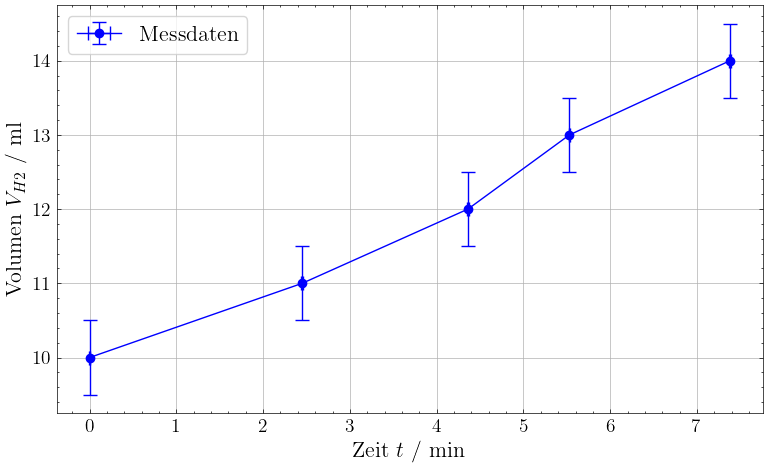
\includegraphics[width=0.6\linewidth]{images/V3_Windkraft_BZelle.png}
    \caption{Gemessene Zeiten $t$ zur Erzeugung von $1 \; \text{ml}$ Wasserstoff in einer Brennstoffzelle beim Betrieb mit Windenergie (blaue Punkte, inklusive Messunsicherheit).
    Die rote Linie zeigt die lineare Ausgleichsgerade der Messdaten zur Bestimmung der gespeicherten Energie pro Minute.}
    \label{fig:V3_WK_Speicher_BZ}
\end{figure}

\noindent Die Energie bzw Menge an Wasserstoff, welche von der Brennstoffzelle in einer Minute gespeichert werden kann, ergibt sich aus der Steigung der Ausgleichsgeraden der Messdaten. Für den Wert der Steigung bzw dem Volumen pro Minute und die Unsicherheit der Größe folgt aus der Regressionsrechnung folgender Wert:
$$\frac{\Delta V_{H2}}{\Delta t} = (0{,}55 \pm 0{,}04) \; \frac{\text{ml}}{\text{min}}$$

\section{Diskussion}

\subsection{Photovoltaik}
\noindent Im ersten Versuch wurde das Verhalten einer Photovoltaikzelle in Abhängigkeit von der Schaltung und dem Abstand zur Lichtquelle untersucht. Bei den Messergebnissen der Leerlaufspannungen $U_{\text{leer}}$ und Kurzschlussströme $I_{\text{kurz}}$, die in Tabelle \ref{tab:MessungenWiderstand} dargestellt sind, zeigte sich, dass sie den theoretischen Erwartungen entsprechen. In der Serienschaltung der beiden Solarzellen addierten sich die Spannungen nahezu ideal, während in der Parallelschaltung die Ströme entsprechend zunahmen. Diese Beobachtung bestätigt das Grundprinzip der Reihenschaltung von Spannungsquellen und der Parallelschaltung von Stromquellen.

\vspace{2mm}

\noindent Wie in Abbildung \ref{fig:V1_PV_Kennlinien} deutlich zu sehen ist, nahm sowohl die Leerlaufspannung als auch der Kurzschlussstrom mit zunehmendem Abstand zwischen Lichtquelle und Photovoltaikmodul ab. Da die erzeugte Spannung und der Strom direkt von der Anzahl an erzeugten Elektron-Loch-Paare abhängen, sinkt mit verringerter Lichtintensität auch die Photostromdichte.

\vspace{2mm}

\noindent Messungenauigkeiten können bei sehr geringen Abständen durch lokale Erwärmung der Zelle oder eine nicht gleichmäßige Beleuchtung auftreten, was die Linearität der Abhängigkeit beeinträchtigen kann. Mögliche Fehlerquellen liegen vor allem in der Positionierung des Solarmoduls und der Ausrichtung der Lichtquelle. Geringe Winkelabweichungen können bereits die effektive Einstrahlungsfläche verändern. Auch die spektrale Zusammensetzung der verwendeten Lichtquelle weicht von der des Sonnenlichts ab, was den Wirkungsgrad beeinflusst.\\
Um für genauere Messergebnisse zu sorgen, könnte in künftigen Messungen die Temperaturabhängigkeit der Solarzelle berücksichtigt werden, da die Leerlaufspannung mit steigender Temperatur typischerweise leicht abnimmt. Insgesamt zeigen die Messergebnisse eine gute qualitative Übereinstimmung mit dem theoretisch erwarteten Verhalten einer Photovoltaikzelle.


\subsection{Brennstoffzelle}
\noindent Im zweiten Versuch wurde der Wirkungsgrad und die Kennlinie einer reversiblen PEM-Brennstoffzelle bestimmt.

\subsubsection{Wirkungsgrad}
\noindent Der Wirkungsgrad ergibt sich aus dem Verhältnis der von der Brennstoffzelle abgegebenen elektrischen Energie \(E_\text{el}\) zur chemisch umgesetzten Energie \(E_\text{chem}\). Der experimentell bestimmte Wirkungsgrad \(\eta = (1.7 \pm 0.4)\;\%\) liegt deutlich unter dem theoretischen Wert von etwa \(50\;\%\), der für eine vergleichbare Brennstoffzelle unter optimalen Betriebsbedingungen mit konstanter Gasversorgung erwartet wird \cite{sfc_wirkungsgrad_brennstoffzelle}.
\vspace{2mm}

\noindent Das deutlich geringere Ergebnis in diesem Versuch ist vor allem auf die sehr niedrige Zellspannung von nur \(U = (80 \pm 4)\,\text{mV}\) und die daraus resultierende geringe elektrische Leistung zurückzuführen. Die Abweichung kann auf Messungenauigkeiten oder defekte Komponenten, etwa einen beschädigten Widerstand \(R\), hindeuten.
Darüber hinaus tragen verschiedene Verlustmechanismen, wie ohmsche Verluste an den Kontakten, Aktivierungsverluste an den Elektroden sowie Konzentrationsverluste infolge unvollständigen Gastransports, zusätzlich zur Verringerung der Effizienz bei.

\subsubsection{Kennlinie}
\noindent Die gemessene Strom-Spannungs-Kennlinie, die in Abbildung \ref{fig:V2_BZ_Kennlinien_Messung} abgebildet ist, zeigt den typischen Verlauf einer Brennstoffzelle mit nahezu linearem Bereich bei kleinen Strömen und einem deutlichen Spannungsabfall bei höheren Stromdichten. Der lineare Fit ergab einen Innenwiderstand von $R_\text{in} = (23{,}6 \pm 1{,}1)\; \text{m}\ohm$ und einer theoretischen Leerlaufspannung von $U_0 = (954 \pm 9) \ \text{mV}$. Die dazugehörige Leistungskurve in Abbildung \ref{fig:V2_BZ_quad_fit_Leistung} kennzeichnet den optimalen Arbeitspunkt der Zelle.
\vspace{2mm}

\noindent Messunsicherheiten ergeben sich aus der Bestimmung des Gasvolumens, möglichen Lecks an den Anschlüssen, sowie Luftblasen in der Brennstoffzelle. Die begrenzte Genauigkeit bei der Strommessung sowie Temperatur- und Feuchtigkeitsschwankungen während des Betriebs können ebenfalls zu Abweichungen führen. Für zukünftige Messungen wäre eine kontinuierliche Aufzeichnung von Spannung und Strom mit höherer zeitlicher Auflösung sowie eine stabilisierte Gasversorgung vorteilhaft. Trotz der geringen Effizienz konnte das Funktionsprinzip der Brennstoffzelle eindeutig bestätigt werden.

\subsection{Windkraft}
\noindent Im dritten Versuchsteil wurde die Umwandlung von Bewegungsenergie des Windes in elektrische Energie untersucht. Die Messung der Leerlaufspannung am Windrad $U_\text{leer}$ in Abhängigkeit von der Gleichspannung an der Windmaschine $U_\text{M}$ ergab eine nahezu lineare Beziehung, welche in Abbildung \ref{fig:V3_WK_fixer_Abstand} zu sehen ist. Dies zeigt, dass die vom Windrad gelieferte Spannung proportional zur Rotationsgeschwindigkeit ist, die wiederum direkt von der Windgeschwindigkeit abhängt.
\vspace{2mm}

\noindent Bei zunehmendem Abstand zwischen Windmaschine und Windrad nahm die Leerlaufspannung erwartungsgemäß ab, da die Luftströmung mit zunehmender Entfernung an Geschwindigkeit verliert und Turbulenzen zunehmen. Dieser Zusammenhang ist in Abbildung \ref{fig:V3_WK_fixe_Spannung} zu erkennen, wobei hier auch zu sehen ist, dass das Maximum der Leerlaufspannung nicht beim kleinsten Abstand liegt sondern in diesem Versuch bei $d=(8{,}00 \pm 0{,}10) \; \text{cm}$ zu finden ist. Dieses Verhalten ist auf strömungstechnische Effekte zurückzuführen. Direkt vor der Windmaschine herrscht eine stark turbulente Strömung mit ungleichmäßigem Druckprofil. Dadurch trifft der Luftstrom nicht gleichmäßig auf die Rotorblätter, was die effektive Anströmgeschwindigkeit und damit die erzeugte Spannung beeinträchtigt. Bei minimal größerem Abstand ist die Strömung bereits etwas stabilisiert und laminarer, was zu einer effizienteren Energieübertragung führt.

\noindent Messunsicherheiten ergeben sich aus der manuellen Einstellung der Abstände, sowie mögliche Reflexionen des Luftstroms an den Versuchsaufbauten, oder der begrenzten Gleichmäßigkeit des erzeugten Luftstroms.

\subsubsection{Elektrisches Potential}
\noindent Zur Untersuchung der Energiespeicherung in Form eines elektrischen Potentials wurde das Windrad an verschiedene Kondensatoren angeschlossen. Die gemessenen Spannungsverläufe, die in den Abbildungen \ref{fig:V3_WK_Fit1}, \ref{fig:V3_WK_Fit2} und \ref{fig:V3_WK_Fit3} angeführt sind, zeigten das erwartete exponentielle Lade- und Entladeverhalten an. Für die drei untersuchten Kondensatoren ergaben sich die in Tabelle \ref{tab:Tau} aufgelisteten Zeitkonstanten $\tau$. Die daraus berechneten Kapazitäten in Tabelle \ref{tab:Capa} stimmen mit den typischen Größenordnungen handelsüblicher Elektrolytkondensatoren überein \cite{tiplermosca}.

\vspace{2mm}

\noindent Die gemessenen Spannungsverläufe stimmen gut mit den berechneten exponentiellen Kurven überein. Dies zeigt, dass der Entladeprozess weitgehend ideal abläuft. Kleine Abweichungen können durch zusätzliche Widerstände in der Schaltung, Leckströme oder Verzögerungen bei der Videoauswertung erklärt werden. Der Versuch veranschaulicht das typische Verhalten eines RC-Kreises und zeigt, dass elektrische Speicher kurzfristige Schwankungen in der Energiezufuhr sehr gut ausgleichen können.

\vspace{2mm}

\noindent Zur Verbesserung der Messgenauigkeit wäre eine direkte Aufzeichnung mit einem Oszilloskop hilfreich, da dadurch der Spannungsverlauf deutlich präziser dargestellt werden kann. Auch die Bestimmung des Innenwiderstandes des Generators würde eine genauere Abschätzung der Energieverluste während des Ladevorgangs ermöglichen.

\subsubsection{Chemisches Potential}
\noindent Im letzten Versuchsteil wurde die vom Windrad erzeugte elektrische Energie genutzt, um eine Brennstoffzelle im Elektrolyse-Betrieb zu betreiben und so chemische Energie in Form von Wasserstoff zu speichern. Die aufgezeichneten Zeiten zur Erzeugung von jeweils 1 ml Wasserstoff zeigen eine konstante Steigung, was auf eine gleichmäßige Leistungsabgabe des Windrades und eine stabile Elektrolyse hinweist. Dieser Vorgang ist in Abbildung \ref{fig:V3_WK_Speicher_BZ} gut zu erkennen. Aus der Regressionsrechnung ergab sich eine mittlere Produktionsrate von $\frac{\Delta V_{H2}}{\Delta t} = (0{,}55 \pm 0{,}04) \; \frac{\text{ml}}{\text{min}}$.

\vspace{2mm}

\noindent Die Effizienz dieser Umwandlung hängt wesentlich von der anliegenden Spannung und der Gasentwicklung an den Elektroden ab. Mögliche Fehlerquellen ergeben sich aus ungleichmäßiger Windzufuhr, Lecks in den Gasleitungen oder der unvollständigen Messung des Gasvolumens aufgrund von Blasenbildung. Eine präzise Kalibrierung der Volumenskala und eine gleichmäßige Windgeschwindigkeit könnten diese Fehler reduzieren.

\newpage
\bibliographystyle{abbrvnat}
\bibliography{lit.bib}

\listoffigures
\listoftables
\end{document}
